\newpage
\subsection{Varmelegeme - Andreas}
\subsubsection{Design}
Der er i løbet af designfasen for varmelegemet fremkommet 2 designtyper. Den ene er brugen af en simpel varmelampe, det andet design er en køleplade med effektmodstande monteret ovenpå for at opvarme selve pladen og derved afgive varme til omgivelserne. Det er besluttet at beholde den sidste idé med effektmodstandene. Dette skyldes nem tilgang til komponenterne der skal bruges, samt en varmelampe bruger 230V som ikke er forbundet til vores system umiddelbart.
Der er for god ordens skyld tilføjet en blæser til at lave en mere ligelig fordeling af varmen.

Det er vurderet at der skal bruges en effekt på 60-80W til opvarmning af miljøet.

\subsubsection{Implementering}
Varmelegemet blev fremstillet med 4 effektmodstande på hver 6.8$\Omega$ og max 50W. Med en 12V strømforsyning og uden hensyn til spændingsfald over en MOSFET transistor, så ender den teoretiske effekt på 84.7W og er simuleret til 82.32W med det simulerede kredsløb på figur \ref{fig:Heater_simulation}.

\begin{figure}[H]
\centering
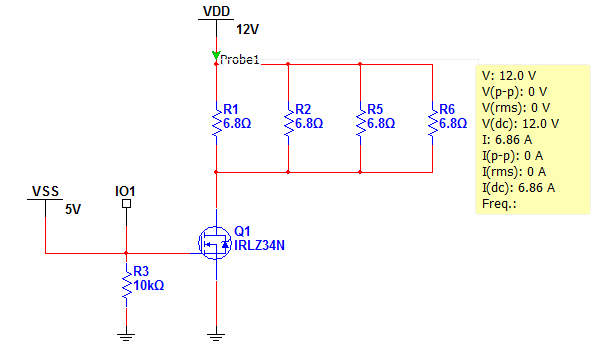
\includegraphics[page=1,width=\linewidth,viewport=-50mm 5mm 180mm 80mm]{./7_projektbeskrivelse/design_og_implementering/hardware/sim_heat.png}
\caption[Figur]{Varmelegeme simuleringskredsløb}
\label{fig:Heater_simulation}
\end{figure}

